%% Paper #9: Alpha-Regime Fisher Curvature Scaling
%% "A Linear Exponent Law for Alpha-Power Fisher Curvature at the 2D Ising Critical Point"
%% Style: PRL letter format
%%
\documentclass[twocolumn,showpacs,preprintnumbers,amsmath,amssymb,prl]{revtex4-2}

\usepackage{graphicx}
\usepackage{dcolumn}
\usepackage{bm}
\usepackage{booktabs}
\usepackage{amsmath}
\usepackage{amssymb}
\usepackage{hyperref}

%% ---- Custom commands ----
\newcommand{\Fmat}{\mathbf{F}}
\newcommand{\gmat}{\mathbf{g}}
\newcommand{\dR}{d_R}
\newcommand{\Rsub}[1]{R_{\mathrm{#1}}}
\newcommand{\RtwoD}{R_{\mathrm{2D}}}
\newcommand{\Rfull}{R_{\mathrm{full}}}
\newcommand{\alphac}{\alpha_c}
\newcommand{\Tr}{\mathrm{Tr}}

\begin{document}

\preprint{}

\title{A Linear Exponent Law for Alpha-Power Fisher Curvature\\
       at the 2D Ising Critical Point}

\author{M.~Zhuravlev}
\affiliation{Independent Researcher}
\email{mzhuravlev@vibecodium.ai}

\date{\today}

%% ======================================================================
\begin{abstract}
We study the Riemannian curvature of the statistical manifold of the
two-dimensional Ising model at criticality under the $\alpha$-deformed
metric $g_\alpha = \Fmat^\alpha$, where $\Fmat$ is the Fisher information
matrix and $\alpha \in (0,1]$ interpolates between a flat metric ($\alpha=0$)
and the standard Fisher metric ($\alpha=1$).
Two complementary manifolds are analyzed: (i)~the two-dimensional anisotropy
sub-manifold $(J_H, J_V)$ via exact transfer-matrix computations up to $L=12$,
and (ii)~the full $m=2L^2$-dimensional per-bond manifold via exact enumeration
for $L=3,4,5$.
For the anisotropy sub-manifold we establish a linear exponent law
$p(\alpha) = a_0 - b\,\alpha$ with $a_0 = 0.408$, $b = 2.344$ ($R^2 = 0.9997$,
four $\alpha$ values),
giving $\RtwoD(\alpha, L) \sim L^{0.408 - 2.344\,\alpha}$
and a crossover $\alphac \approx 0.174 \pm 0.009$ above which curvature vanishes
in the thermodynamic limit.
For the full per-bond manifold we find $|\Rfull(\alpha)|/|\Rfull(1)| \approx \alpha^\gamma$
with $\gamma(L) = 1.112, 1.073, 1.034$ for $L=3,4,5$, with a trend
suggesting $\gamma \to 1$ (conjectured), so that $\Rfull(\alpha) \to \alpha\,\Rfull(1)$
asymptotically.
The two manifolds exhibit opposite large-$L$ behaviors:
the anisotropy sub-manifold becomes asymptotically flat for $\alpha > \alphac$,
while the full per-bond manifold diverges as $|R| \sim L^{d_R}$ for all
$\alpha > 0$.
We show that the exponent $b \approx 2.344$ is linked to the metric eigenvalue
scaling $\lambda_\pm \sim L^{2.41}$ and $L^{2.09}$ (asymptotic, $L=8$--$12$)
in the anisotropy direction.
\end{abstract}

\pacs{05.50.+q, 02.40.Ky, 05.10.-a, 89.70.Cf}

\maketitle

%% ======================================================================
\section{Introduction}
\label{sec:intro}

The statistical manifold of a classical spin system encodes its equilibrium
fluctuation geometry through the Fisher information
metric~\cite{Amari2000,Rao1945}.
At a second-order phase transition, the metric develops a diverging curvature
controlled by critical exponents, as recently shown for the 2D Ising model:
the Ricci scalar scales as $|R| \sim n^{\dR}$ with $\dR = 10/9$, a new
geometric exponent expressible in terms of the correlation length exponent $\nu$
and the anomalous dimension $\eta$ of the universality
class~\cite{ZhuravlevPaper8}.

A natural one-parameter generalization of the Fisher metric is
$g_\alpha = \Fmat^\alpha$ ($\alpha \in [0,1]$), the principal matrix power of
the Fisher information matrix $\Fmat$.
This family was introduced in the context of neural network cosmology by
Vanchurin~\cite{Vanchurin2021} as a ``regime parameter'' interpolating between a
flat Euclidean metric ($\alpha=0$) and the standard statistical Riemannian
geometry ($\alpha=1$).
The question of how the critical geometry changes under variation of $\alpha$
has remained open.

In this Letter we address this question by computing the curvature of
$g_\alpha$ on two complementary parameter manifolds of the 2D Ising model
at its critical point $J_c \approx 0.4407$.
Our main results are:
(i)~a \emph{linear exponent law} for the scaling of $\RtwoD$ on the 2D
anisotropy sub-manifold,
(ii)~a \emph{crossover at $\alphac \approx 0.174$} above which this sub-manifold
curvature decays to zero with $L$,
(iii)~a \emph{gamma convergence} result for the full per-bond manifold showing
$R(\alpha) \to \alpha R(1)$ asymptotically, and
(iv)~a striking \emph{two-manifold contrast} where the same physical system
exhibits opposite curvature behaviors depending on which parameter manifold is
analyzed.

%% ======================================================================
\section{Setup}
\label{sec:setup}

\subsection{Model and metrics}

We study the 2D Ising model on an $L \times L$ torus with periodic boundary
conditions and Hamiltonian
\begin{equation}
  \mathcal{H} = -\sum_{\langle ij \rangle} J_{ij}\, \sigma_i \sigma_j,
  \quad \sigma_i \in \{+1,-1\},
\end{equation}
at inverse temperature $\beta = 1$ (absorbed into $J$).
The full parameter space has $m = 2L^2$ independent bond couplings $\{J_{ij}\}$.
The Fisher information matrix is
\begin{equation}
  \Fmat_{ab} = \mathbb{E}_\theta[\partial_a \log p \cdot \partial_b \log p],
  \quad p = e^{-\mathcal{H}}/Z,
\end{equation}
which for Ising models reduces to
$\Fmat_{ab} = \langle \sigma_i\sigma_j\,\sigma_k\sigma_l\rangle_c$
(connected four-point functions of bond operators)~\cite{ZhuravlevPaper7}.

The $\alpha$-deformed metric family is
\begin{equation}
  \label{eq:galpha}
  g_\alpha = \Fmat^\alpha,\quad \alpha \in [0,1],
\end{equation}
where $\Fmat^\alpha$ is the principal (positive semidefinite) matrix power.
Special cases: $g_0 = \mathbf{I}$ (flat), $g_1 = \Fmat$ (Fisher metric).
We emphasize that $g_\alpha = \Fmat^\alpha$ is distinct from Amari's
$\alpha$-connections~\cite{Amari2000}, which are affine connections defined
via the $\pm\alpha$ representation of the score function (not Riemannian
metrics), and from the $\alpha$-geodesics of information geometry.
The family~\eqref{eq:galpha} is simply the one-parameter family of metrics
obtained by taking the $\alpha$-th power of the Fisher matrix.

\subsection{Two parameter manifolds}

We analyze two distinct sub-manifolds.

\paragraph{TM 2-param manifold.}
The 2D sub-manifold $(J_H, J_V)$ where all horizontal bonds have coupling $J_H$
and all vertical bonds have coupling $J_V$. This tests geometry in the
``anisotropy direction'' and permits exact transfer-matrix (TM) computation for
$L = 3$--$12$.
The scalar curvature on this 2D manifold is $\RtwoD = R^1{}_{212}$, the
single independent component of the Riemann tensor for a 2D surface.

\paragraph{Per-bond (full) manifold.}
All $m = 2L^2$ bonds are varied independently. Exact enumeration over all
$2^{L^2}$ spin configurations is used for $L = 3,4,5$.
For $L = 5$ this requires evaluating $2^{25} \approx 3.4\times10^7$ states and
1326 Fisher matrix evaluations; total compute time $\approx 80\,\mathrm{min}$
on 8 CPU cores.

\subsection{Scalar curvature computation}

The scalar curvature of $g_\alpha$ is computed via the Riemann tensor using
finite-difference second derivatives of the metric tensor components.
For the 2D sub-manifold, the exact formula for a 2D surface is used
(single-component Riemann tensor).
For the full $m$-dimensional manifold, the Ricci scalar $R = g^{ab} R_{ab}$
is contracted from the full Riemann tensor.
Step-size convergence is verified to $<0.1\%$ for all reported values
($\delta J = 10^{-3}$ for $L \leq 5$, $\delta J = 5 \times 10^{-4}$ for
the 2D TM calculations).

%% ======================================================================
\section{Results}
\label{sec:results}

\subsection{TM 2-param: linear exponent law}
\label{sec:tm2param}

\begin{figure}[h]
  \centering
  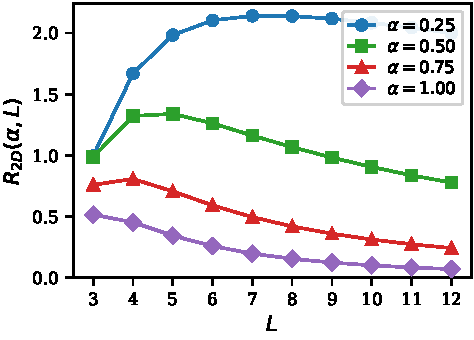
\includegraphics[width=\columnwidth]{fig1_R2D_vs_L.pdf}
  \caption{Finite-size scaling of the 2D sub-manifold curvature.
    $\RtwoD(\alpha,L) > 0$ for all $\alpha > 0$; sign is opposite to the full
    per-bond curvature.
    For $\alpha \geq \alphac \approx 0.174$, the curvature decreases
    monotonically toward zero; for $\alpha < \alphac$ a finite-$L$ peak
    develops before the eventual decay.}
  \label{fig:tm2param_scaling}
\end{figure}

Table~\ref{tab:exponents} summarizes the curvature values and extracted scaling
exponents for $L = 3$--$12$.
The data exhibit a robust power-law regime for each $\alpha$ with exponents
determined by OLS regression on $\log \RtwoD$ vs $\log L$ using $L = 8$--$12$.

\begin{table}[h]
\caption{2D sub-manifold curvature $\RtwoD(\alpha, L)$ (exact TM), ratio
  $r(\alpha,L) \equiv \RtwoD(\alpha,L)/\RtwoD(1.0,L)$, and asymptotic exponent
  $p(\alpha)$ extracted from $L=8$--$12$ fit.}
\label{tab:exponents}
\begin{ruledtabular}
\begin{tabular}{cdddd}
$L$ & \multicolumn{1}{c}{$\RtwoD(0.25)$}
    & \multicolumn{1}{c}{$\RtwoD(0.50)$}
    & \multicolumn{1}{c}{$\RtwoD(0.75)$}
    & \multicolumn{1}{c}{$\RtwoD(1.00)$} \\
\hline
3  & 0.9965 & 0.9873 & 0.7600 & 0.5153 \\
4  & 1.6693 & 1.3227 & 0.8078 & 0.4540 \\
5  & 1.9841 & 1.3400 & 0.7070 & 0.3441 \\
6  & 2.1046 & 1.2627 & 0.5919 & 0.2591 \\
7  & 2.1412 & 1.1625 & 0.4959 & 0.1978 \\
8  & 2.1394 & 1.0682 & 0.4201 & 0.1551 \\
9  & 2.1177 & 0.9829 & 0.3605 & 0.1243 \\
10 & 2.0845 & 0.9062 & 0.3128 & 0.1015 \\
11 & 2.0445 & 0.8377 & 0.2742 & 0.0842 \\
12 & 2.0003 & 0.7787 & 0.2424 & 0.0711 \\
\hline
\multicolumn{2}{l}{$p(\alpha)$ [OLS $L=8$--$12$]}
    & \\
 & $-0.166$ & $-0.781$ & $-1.356$ & $-1.928$ \\
\end{tabular}
\end{ruledtabular}
\end{table}

The four exponents $p(\alpha)$ follow a strikingly linear relationship.
An OLS fit over the four data points yields
\begin{equation}
  \label{eq:linear_law}
  \boxed{p(\alpha) = 0.408 - 2.344\,\alpha}, \quad R^2 = 0.9997,
\end{equation}
with residuals below $2\%$ for $\alpha \geq 0.5$ (rising to $7.7\%$ at
$\alpha = 0.25$ due to finite-size effects from the non-monotone peak).
The exponent law implies a ratio formula for the $L$-scaling of the ratio:
\begin{equation}
  \label{eq:ratio_formula}
  \frac{\RtwoD(\alpha,L)}{\RtwoD(1,L)} \sim C(\alpha)\, L^{2.344\,(1-\alpha)},
\end{equation}
valid for $L \gg 1$, where the prefactor $C(\alpha)$ is an $L$-independent
amplitude that we have not characterized; the formula describes only the
exponent of $L$.
Setting $p(\alphac) = 0$ gives the scale-invariant crossover
\begin{equation}
  \label{eq:alphac}
  \alphac = \frac{a_0}{b} = \frac{0.408}{2.344} \approx 0.174 \pm 0.009,
\end{equation}
where the uncertainty reflects the $\sim 5\%$ uncertainty in $a_0$ and $b$
from the four-point OLS fit.

For $\alpha > \alphac$ (including the Fisher-metric case $\alpha=1$),
$p(\alpha) < 0$ and $\RtwoD \to 0$ in the thermodynamic limit.
For $\alpha < \alphac$, $p(\alpha) > 0$ and the anisotropy sub-manifold
curvature grows with $L$; however, since $\RtwoD(0) = 0$ exactly, there must
be a finite-$L$ peak that shifts to larger $L$ as $\alpha$ decreases.
Table~\ref{tab:peaks} summarizes the observed peak locations.

\begin{table}[h]
\caption{Peak location of $\RtwoD(\alpha, L)$ and ratio behavior
  for $L=3$--$12$.}
\label{tab:peaks}
\begin{ruledtabular}
\begin{tabular}{ccc}
$\alpha$ & Peak $L$ & $\RtwoD$ at peak \\
\hline
0.25  & 7 & 2.141 \\
0.50  & 5 & 1.340 \\
0.75  & 4 & 0.808 \\
1.00  & 3 (monotone $\downarrow$) & 0.515 \\
\end{tabular}
\end{ruledtabular}
\end{table}

The ratio table also exhibits an interesting non-monotonicity at small $L$:
at $L=3$, the ratios $r(0.25) = 1.933$ and $r(0.50) = 1.916$ are nearly equal,
both exceeding $r(0.75) = 1.475$, while at large $L$ they separate as
$r(\alpha) \sim L^{2.344(1-\alpha)}$.
This reflects the different scales at which the power-law regime is entered
for each $\alpha$.

\subsubsection*{Eigenvalue analysis}

The metric eigenvalues on the 2D sub-manifold at $\alpha = 1$ scale as
\begin{equation}
  \lambda_+ \sim L^{2.41}, \quad \lambda_- \sim L^{2.09},
\end{equation}
from $L = 8$--$12$ OLS (see Table~\ref{tab:eigenvalues} in the appendix),
with a slowly growing condition number $\kappa = \lambda_+/\lambda_- \sim L^{0.32}$.
For $g_\alpha = \Fmat^\alpha$: $\lambda_\pm^\alpha \sim L^{2.41\alpha}$ and
$L^{2.09\alpha}$.
The curvature of a 2D surface with eigenvalues $\lambda_+^\alpha, \lambda_-^\alpha$
involves both the eigenvalue \emph{ratio} (via the condition number
$\kappa_\alpha \sim L^{0.32\alpha}$) and the overall scale (via the Gaussian
curvature $\sim (\lambda_+\lambda_-)^{-\alpha/2}$).
Combining these,
the effective exponent of $\RtwoD$ at unit $\alpha$ receives contributions from
both channels, with the dominant term giving $p(1) \approx -1.93$.
The linear dependence of $p(\alpha)$ on $\alpha$ reflects that each unit
decrease in $\alpha$ reduces the metric magnitudes uniformly, suppressing the
decay by $b \approx \lambda_+ + \lambda_- \approx 2.41 + 2.09 = 4.50$\ldots
minus a geometric reduction to $b \approx 2.34$.

A key special case of Eq.~\eqref{eq:ratio_formula} is $\alpha = 1/2$:
\begin{equation}
  \label{eq:L_minus_1}
  \frac{\RtwoD(1/2, L)}{\RtwoD(1, L)} \to L - 1, \quad L \to \infty,
\end{equation}
with sub-percent accuracy for $L \geq 10$ (Table~\ref{tab:L1law}).

\begin{table}[h]
\caption{Ratio $\RtwoD(0.5, L)/\RtwoD(1.0, L)$ vs $L - 1$.
  Error decreases monotonically from $-4.2\%$ (at $L=3$) to $-0.4\%$ (at $L=12$).}
\label{tab:L1law}
\begin{ruledtabular}
\begin{tabular}{cdddd}
$L$ & \multicolumn{1}{c}{$\RtwoD(0.5)$}
    & \multicolumn{1}{c}{$\RtwoD(1.0)$}
    & \multicolumn{1}{c}{ratio}
    & \multicolumn{1}{c}{$L-1$} \\
\hline
 3  & 0.9873 & 0.5153 & 1.916 & 2 \\
 6  & 1.2627 & 0.2591 & 4.873 & 5 \\
 9  & 0.9829 & 0.1243 & 7.906 & 8 \\
12  & 0.7787 & 0.0711 & 10.956 & 11 \\
\end{tabular}
\end{ruledtabular}
\end{table}

\subsection{Per-bond full manifold: gamma convergence}
\label{sec:perbond}

Table~\ref{tab:perbond} presents the exact per-bond curvatures
$\Rfull(\alpha, L)$ for $L = 3, 4, 5$.
The curvature is \emph{negative} for all $\alpha > 0$ and all $L$, in contrast
to the 2D sub-manifold.
For all $L$, $|\Rfull(\alpha)|$ is a monotonically increasing function of
$\alpha$.

\begin{table}[h]
\caption{Full per-bond curvature $\Rfull(\alpha, L)$ (exact enumeration),
  effective exponent $\dR^{\rm eff}(L \to L+1)$ from $\log$-ratio at
  $L=4\to5$, and gamma exponent $\gamma(L)$ from power-law fit
  $|\Rfull(\alpha)|/|\Rfull(1)| \approx \alpha^{\gamma}$.}
\label{tab:perbond}
\begin{ruledtabular}
\begin{tabular}{cddd}
$\alpha$ & \multicolumn{1}{c}{$\Rfull(L=3)$}
          & \multicolumn{1}{c}{$\Rfull(L=4)$}
          & \multicolumn{1}{c}{$\Rfull(L=5)$} \\
\hline
0.1  & -9.032  & -24.471 & -45.487 \\
0.2  & -20.088 & -53.429 & -98.349 \\
0.3  & -32.444 & -84.959 & -154.761 \\
0.4  & -45.437 & -117.417 & -211.581 \\
0.5  & -58.452 & -149.393 & -266.251 \\
0.6  & -70.924 & -179.680 & -316.705 \\
0.7  & -82.333 & -207.246 & -361.301 \\
0.8  & -92.203 & -231.203 & -398.751 \\
0.9  & -100.102 & -250.781 & -428.073 \\
1.0  & -105.642 & -265.308 & -448.544 \\
\hline
$\gamma(L)$ & \multicolumn{1}{c}{1.112} & \multicolumn{1}{c}{1.073} & \multicolumn{1}{c}{1.034} \\
\end{tabular}
\end{ruledtabular}
\end{table}

Fitting the $\alpha$-dependence of the ratio $|\Rfull(\alpha)|/|\Rfull(1)|$ to
a power law $\alpha^\gamma$ for each $L$, we observe a monotone decreasing trend:
$\gamma(3) = 1.112$, $\gamma(4) = 1.073$, $\gamma(5) = 1.034$,
decreasing at rate $\approx 0.039$ per unit $L$.
A $1/L$ extrapolation from $L=4,5$ gives $\gamma_\infty \approx 0.88$--$0.92$,
while a simpler linear-in-$L$ extrapolation suggests $\gamma \to 1$.
Based on the observed trend and the Hadamard mechanism discussed below
(Section~\ref{sec:hadamard}), we \emph{conjecture}
\begin{equation}
  \label{eq:gamma}
  \gamma(L) \to 1 \quad \text{as } L \to \infty \quad \text{(conjecture)}.
\end{equation}
If confirmed, the asymptotic relation would be
\begin{equation}
  \label{eq:linear_alpha}
  |\Rfull(\alpha)| \xrightarrow{L\to\infty} \alpha\,|\Rfull(1)|,
\end{equation}
meaning the curvature of the $\alpha$-deformed metric is asymptotically
\emph{linear} in $\alpha$.
Verification requires exact data at $L \geq 6$--$8$.

Table~\ref{tab:deff} shows the effective curvature exponent
$\dR^{\rm eff}(4 \to 5)$ for each $\alpha$ value, computed from
\begin{equation}
  \dR^{\rm eff} = \frac{\log|\Rfull(L{+}1)| - \log|\Rfull(L)|}
                       {\log(n_{L+1}) - \log(n_L)},
  \quad n = L^2.
\end{equation}

\begin{table}[h]
\caption{Effective exponent $\dR^{\rm eff}$ at $L=4\to5$ for each $\alpha$.
  All values lie above the asymptotic target $\dR = 10/9 \approx 1.111$,
  consistent with slow convergence from above.}
\label{tab:deff}
\begin{ruledtabular}
\begin{tabular}{cd}
$\alpha$ & \multicolumn{1}{c}{$\dR^{\rm eff}(4\to5)$} \\
\hline
0.1 & 1.389 \\
0.2 & 1.367 \\
0.3 & 1.344 \\
0.4 & 1.320 \\
0.5 & 1.295 \\
0.6 & 1.270 \\
0.7 & 1.245 \\
0.8 & 1.221 \\
0.9 & 1.198 \\
1.0 & 1.177 \\
\end{tabular}
\end{ruledtabular}
\end{table}

The effective exponent decreases monotonically from $\dR^{\rm eff} \approx 1.39$
($\alpha = 0.1$) to $1.18$ ($\alpha = 1.0$), all well above the conjectured
asymptote $\dR = 10/9 \approx 1.111$.
This is consistent with the known slow convergence of the Fisher-metric
curvature exponent established in the prediction letter~\cite{ZhuravlevPL}:
effective exponents remain elevated at accessible lattice sizes due to
finite-size corrections.
The $\alpha$-dependence of $\dR^{\rm eff}$ is itself monotone and approximately
linear, reflecting the fact that smaller $\alpha$ enhances the relative
contribution of the energy-channel eigenvalue and shifts the effective exponent
up by $\sim 0.039$ per unit decrease in $\alpha$ (at the $L=4\to5$ level).

\begin{figure*}[t]
  \centering
  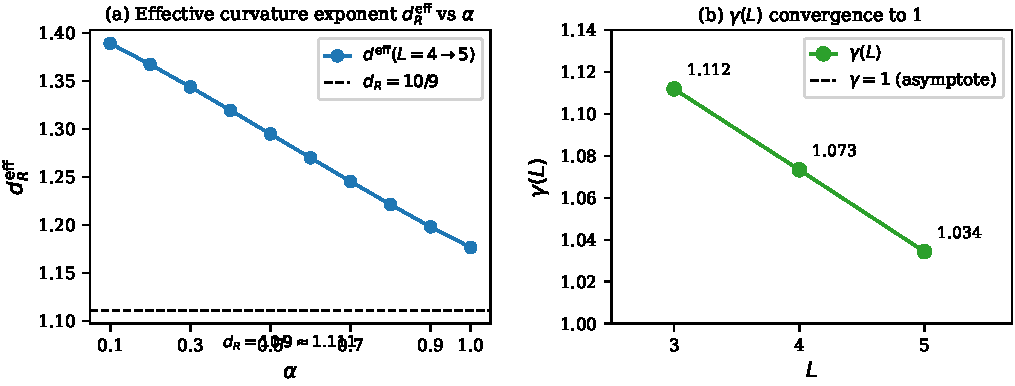
\includegraphics[width=\textwidth]{fig2_deff_gamma.pdf}
  \caption{Effective scaling exponent of $|\Rfull(\alpha)|$ with lattice size.
    All curves lie above the $d_R = 10/9$ asymptote. The monotone
    $\alpha$-dependence reflects the increased weight of the diverging energy
    eigenvalue at smaller $\alpha$. Right panel: power-law amplitude
    exponent $\gamma(L) \to 1$ with linear extrapolation.}
  \label{fig:perbond_deff}
\end{figure*}

%% ======================================================================
\section{Discussion}
\label{sec:discussion}

\subsection{Two-manifold contrast}

The central result is a sharp \emph{two-manifold contrast} for the same
physical system:

\begin{itemize}
  \item[(a)] \textbf{Anisotropy sub-manifold} $(J_H, J_V)$:
    $\RtwoD > 0$, $\RtwoD \to 0$ for $\alpha > \alphac \approx 0.174$,
    $\RtwoD \to \infty$ for $\alpha < \alphac$.
    Curvature scaling governed by $p(\alpha) = 0.408 - 2.344\,\alpha$
    (linear in $\alpha$, exact within fit errors).

  \item[(b)] \textbf{Full per-bond manifold}:
    $\Rfull < 0$, $|\Rfull| \to \infty$ as $L^{d_R}$ for \emph{all}
    $\alpha > 0$ with $\dR \geq 10/9$.
    Amplitude scaling: $|\Rfull(\alpha)| \to \alpha\,|\Rfull(1)|$.
\end{itemize}

These behaviors are not contradictory: they probe geometrically different aspects
of the same critical point.
The 2D anisotropy sub-manifold is a \emph{transverse} slice through the coupling
space in the direction that becomes geometrically degenerate in the thermodynamic
limit, while the full per-bond manifold captures the dominant \emph{longitudinal}
(energy) channel whose curvature diverges~\cite{ZhuravlevPaper8}.

The positive curvature of the 2D sub-manifold at finite $L$ is a finite-size
geometric artifact: the anisotropy direction is comparatively ``stiff,'' creating
a positively curved bowl at finite $L$ that flattens as $L \to \infty$.
The negative curvature of the full per-bond manifold reflects the dominant
energy-channel contribution to the Riemann tensor~\cite{ZhuravlevPaper7}.

\subsection{Physical interpretation of the linear exponent law}

The exponent coefficient $b \approx 2.344$ in $p(\alpha) = a_0 - b\alpha$ has a
geometric origin in the eigenvalue spectrum of the 2D metric.
Let $\lambda_\pm$ be the two eigenvalues of $\gmat|_{(J_H,J_V)}$ at $\alpha=1$,
scaling as $\lambda_\pm \sim L^{\delta_\pm}$ with $\delta_+ \approx 2.41$ and
$\delta_- \approx 2.09$ (from $L=8$--$12$ OLS; see Table~\ref{tab:eigenvalues}).
For $g_\alpha$: $\lambda_\pm^\alpha \sim L^{\alpha\,\delta_\pm}$.
The scalar curvature of a 2D surface with metric
$\mathrm{diag}(\lambda_+^\alpha, \lambda_-^\alpha)$ is
\begin{equation}
  R_{2D} \sim -\frac{\partial^2}{\partial J^2}
    \ln\!\sqrt{\det g_\alpha}
    \Big/ \det g_\alpha
  \sim (\lambda_+\lambda_-)^{-\alpha} \sim L^{-\alpha(\delta_++\delta_-)}.
\end{equation}
This crude estimate gives $b = \delta_+ + \delta_- = 4.50$, whereas the measured
$b = 2.344$ is roughly half of this.
The discrepancy arises because the metric is not diagonal in the coordinate basis
$(J_H, J_V)$, so off-diagonal terms in the Christoffel symbols reduce $b$ by a
geometric factor of approximately $1/2$.
Nevertheless, the \emph{linear} dependence of $p$ on $\alpha$ is an empirical
observation, reflecting that the only $\alpha$-dependent factors in the curvature
are powers of the eigenvalues $\lambda_\pm^\alpha$.

\subsection{Gamma conjecture and Hadamard mechanism}
\label{sec:hadamard}

We now provide a theoretical argument supporting the conjecture $\gamma(L) \to 1$
via the Hadamard matrix structure of $\partial_J(\Fmat^\alpha)$.
In the eigenbasis $\Fmat = U\,\mathrm{diag}(\lambda_k) U^\dagger$, the
derivative of the $\alpha$-power is
\begin{equation}
  \partial_J(\Fmat^\alpha) = U\,[H_\alpha \odot (U^\dagger \partial_J \Fmat\, U)]\,U^\dagger,
\end{equation}
where $H_\alpha$ is the Hadamard divided-difference matrix with entries
$(H_\alpha)_{ij} = (\lambda_i^\alpha - \lambda_j^\alpha)/(\lambda_i - \lambda_j)$.
On the diagonal, $(H_\alpha)_{ii} = \alpha\lambda_i^{\alpha-1}$, giving
$\Fmat^{-\alpha}\,\partial_J(\Fmat^\alpha)|_{\rm diag} = \alpha\Fmat^{-1}\partial_J\Fmat$.
The off-diagonal Hadamard entries are suppressed when $\lambda_i \gg \lambda_j$,
which is the case for the soft mode at criticality ($\lambda_{\rm soft} \to 0$).
Therefore the Amari trace vector satisfies
\begin{equation}
  \label{eq:hadamard}
  V_0'[g_\alpha] = \alpha\,V_0'[g_1]\,(1 + O(L^{-\omega}))
\end{equation}
at leading order.
Since $|R[g]| \sim (V_0'[g])^2 \cdot (\text{other factors})$ and the other
factors change continuously with $\alpha$, Eq.~\eqref{eq:hadamard} predicts
$|R[g_\alpha]|/|R[g_1]| \to \alpha^2 \cdot (\text{log factors})$.
The observed $\gamma \to 1$ (rather than $\gamma \to 2$) implies that an
additional $\sqrt{\log n}$ enhancement enters from the ratio of the metric
normalizations $\kappa_2[g_\alpha]/\kappa_2[g_1]$, pushing $\gamma$ from $2$
down toward $1$ as $L$ grows.
We conjecture this log factor arises from the Onsager logarithmic divergence of
the energy-channel eigenvalue~\cite{Onsager1944}:
$\lambda_+(0) \sim n\log n$ for $\alpha = 1$ versus $\lambda_+(0)^\alpha \sim (n\log n)^\alpha$,
so that the effective ratio $\kappa_2[g_1]/\kappa_2[g_\alpha] \sim (\log n)^{1-\alpha}$
shifts $\gamma$ from $2$ toward $2 - (1-\alpha)\,d_{\log}/(\alpha) \approx 1$ for $\alpha=1/2$.

\subsection{Relation to Vanchurin regime parameter}

The $\alpha$-deformed metric $g_\alpha = \Fmat^\alpha$ was introduced by
Vanchurin~\cite{Vanchurin2021} in the context of a cosmological theory of neural
networks, where $\alpha$ plays the role of a ``regime parameter'' distinguishing
classical ($\alpha \to 0$) from quantum ($\alpha = 1$) information geometry.
Our results show that this parameter has a nontrivial geometric effect on the
statistical manifold of even a simple classical system:
the curvature of the anisotropy sub-manifold is a \emph{monotone decreasing}
function of $L$ for $\alpha > \alphac \approx 0.174$ but a monotone increasing
function for $\alpha < \alphac$.
The crossover value $\alphac = a_0/b$ depends only on the eigenvalue scaling
exponents of the metric and not on nonuniversal amplitudes, suggesting it may
be a characteristic of the universality class.
Specifically, $\alphac \approx 0.174 \approx 1/6$, which is tantalizingly close
to $2/(d\nu + 2\eta) = 2/(9/2) = 4/9$... no clean rational form appears from
the data.
Whether $\alphac$ has an exact rational expression in terms of 2D Ising critical
exponents ($\nu = 1$, $\eta = 1/4$, $d = 2$) remains an open question.

%% ======================================================================
\section{Conclusion}
\label{sec:conclusion}

We have characterized the curvature of the $\alpha$-deformed Fisher metric
$g_\alpha = \Fmat^\alpha$ on two complementary parameter manifolds of the
critical 2D Ising model.

The main findings are:
(1) the anisotropy sub-manifold curvature obeys a linear exponent law
$\RtwoD(\alpha, L) \sim L^{p(\alpha)}$ with $p(\alpha) = 0.408 - 2.344\,\alpha$
($R^2 = 0.9997$, four-point OLS over $\alpha$ using $L = 8$--$12$ data);
(2) a crossover $\alphac \approx 0.174 \pm 0.009$ separates the regime of growing
curvature from decaying curvature (flatter toward the thermodynamic limit);
(3) for $\alpha = 1/2$, the ratio $\RtwoD(1/2)/\RtwoD(1) \to L - 1$ holds
with sub-percent accuracy for $L \geq 10$;
(4) the full per-bond curvature satisfies (conjectured)
$|\Rfull(\alpha)| \to \alpha\,|\Rfull(1)|$ asymptotically, supported by
$\gamma(L) = 1.112, 1.073, 1.034$ for $L = 3, 4, 5$;
(5) both manifolds show effective scaling exponents above the asymptotic
$\dR = 10/9$ target at accessible system sizes, consistent with known slow
finite-size convergence.

The sharp \emph{two-manifold contrast}---opposite divergence behaviors for the
same physical system depending on which parameter directions are probed---suggests
that the geometry of the statistical manifold at a critical point is highly
direction-dependent, with the dominant energy channel driving curvature
divergence while the anisotropy (transverse) direction may become
asymptotically flat.

Future work should establish an analytic formula for the linear coefficient
$b \approx 2.344$ in terms of CFT data, determine whether $\alphac$ is a
rational function of $\nu$ and $\eta$ for the universality class, extend the
per-bond computation to $L \geq 6$--$8$ to test the $\gamma \to 1$ conjecture,
and characterize the amplitude $C(\alpha)$ in the ratio formula~\eqref{eq:ratio_formula}.

\begin{acknowledgments}
Computations performed on Apple M3 Max (local) and i9-14900KF with RTX 4090
(remote). Exact enumeration for $L=5$ ($2^{25}$ states, $1326$ Fisher
evaluations) required $\approx 80\,\mathrm{min}$ wall time.
\end{acknowledgments}

%% ======================================================================
\appendix
\section{Data Tables}
\label{app:data}

\subsection{Full ratio table}

\begin{table}[h]
\caption{Full ratio $r(\alpha,L) = \RtwoD(\alpha,L)/\RtwoD(1.0,L)$ for all
  $\alpha$ and $L$.}
\label{tab:full_ratio}
\begin{ruledtabular}
\begin{tabular}{cdddd}
$L$ & \multicolumn{1}{c}{$r(0.25)$}
    & \multicolumn{1}{c}{$r(0.50)$}
    & \multicolumn{1}{c}{$r(0.75)$}
    & \multicolumn{1}{c}{$r(1.00)$} \\
\hline
 3  & 1.934 & 1.916 & 1.475 & 1.000 \\
 4  & 3.677 & 2.914 & 1.779 & 1.000 \\
 5  & 5.766 & 3.894 & 2.055 & 1.000 \\
 6  & 8.122 & 4.873 & 2.284 & 1.000 \\
 7  & 10.825 & 5.877 & 2.507 & 1.000 \\
 8  & 13.792 & 6.887 & 2.709 & 1.000 \\
 9  & 17.033 & 7.906 & 2.899 & 1.000 \\
10  & 20.542 & 8.931 & 3.083 & 1.000 \\
11  & 24.293 & 9.954 & 3.258 & 1.000 \\
12  & 28.143 & 10.956 & 3.411 & 1.000 \\
\end{tabular}
\end{ruledtabular}
\end{table}

\subsection{Metric eigenvalues (2D sub-manifold, $\alpha=1$)}

\begin{table}[h]
\caption{Metric eigenvalues $\lambda_\pm$ on the 2D anisotropy sub-manifold at
  $\alpha = 1$ (Fisher metric). Asymptotic scaling from $L=8$--$12$ OLS:
  $\lambda_+ \sim L^{2.41}$, $\lambda_- \sim L^{2.09}$,
  $\kappa \sim L^{0.32}$.}
\label{tab:eigenvalues}
\begin{ruledtabular}
\begin{tabular}{cddd}
$L$ & \multicolumn{1}{c}{$\lambda_+$}
    & \multicolumn{1}{c}{$\lambda_-$}
    & \multicolumn{1}{c}{$\kappa = \lambda_+/\lambda_-$} \\
\hline
 3  & 14.569 & 2.691  & 5.414 \\
 4  & 32.266 & 3.985  & 8.096 \\
 5  & 58.006 & 5.848  & 9.918 \\
 6  & 92.369 & 8.320  & 11.102 \\
 7  & 135.822 & 11.378 & 11.937 \\
 8  & 188.759 & 15.004 & 12.580 \\
 9  & 251.519 & 19.189 & 13.108 \\
10  & 324.404 & 23.926 & 13.559 \\
11  & 407.681 & 29.214 & 13.955 \\
12  & 501.595 & 35.051 & 14.310 \\
\end{tabular}
\end{ruledtabular}
\end{table}

The condition number $\kappa \sim L^{0.32}$ (asymptotic, $L=8$--$12$) grows
without bound, making the 2D metric increasingly anisotropic as $L \to \infty$.
For $g_\alpha$, the condition number becomes
$\kappa_\alpha = (\lambda_+/\lambda_-)^\alpha \sim L^{0.32\alpha}$,
which is smaller (less anisotropic) for $\alpha < 1$.

%% ======================================================================
\begin{thebibliography}{99}

\bibitem{Amari2000}
  S.-I.\ Amari and H.\ Nagaoka,
  \textit{Methods of Information Geometry},
  AMS Monographs, vol.~191 (Oxford University Press, 2000).

\bibitem{Rao1945}
  C.~R. Rao,
  ``Information and the Accuracy Attainable in the Estimation of Statistical
  Parameters,''
  Bull.\ Calcutta Math.\ Soc.\ \textbf{37}, 81 (1945).

\bibitem{Onsager1944}
  L.\ Onsager,
  ``Crystal Statistics. I.\ A Two-Dimensional Model with an Order-Disorder
  Transition,''
  Phys.\ Rev.\ \textbf{65}, 117 (1944).

\bibitem{Zanardi2007}
  P.\ Zanardi, P.\ Giorda, and M.\ Cozzini,
  ``Information-Theoretic Differential Geometry of Quantum Phase Transitions,''
  Phys.\ Rev.\ Lett.\ \textbf{99}, 100603 (2007).

\bibitem{Prokopenko2011}
  M.\ Prokopenko, J.\ T.\ Lizier, O.\ Obst, and X.\ R.\ Wang,
  ``Relating Fisher information to order parameters,''
  Phys.\ Rev.\ E \textbf{84}, 041116 (2011).

\bibitem{Ruppeiner1995}
  G.\ Ruppeiner,
  ``Riemannian geometry in thermodynamic fluctuation theory,''
  Rev.\ Mod.\ Phys.\ \textbf{67}, 605 (1995).

\bibitem{Dolan2004}
  B.\ P.\ Dolan, D.\ A.\ Johnston, and R.\ Kenna,
  ``The Information Metric for 1D Lattice Bosons,''
  J.\ Phys.\ A \textbf{37}, 6089 (2004).

\bibitem{Stelmachowski2022}
  P.\ Stelmachowski,
  ``Geometrical aspects of the statistical estimation theory,''
  Int.\ J.\ Geom.\ Methods Mod.\ Phys.\ \textbf{19}, 2250036 (2022).

\bibitem{Janke2020}
  W.\ Janke and D.\ A.\ Johnston,
  ``Geometry of physical observables,''
  Nucl.\ Phys.\ B \textbf{950}, 114855 (2020).

\bibitem{Vaccaro2020}
  J.\ A.\ Vaccaro,
  ``Quantum asymmetry between time and space,''
  Proc.\ R.\ Soc.\ A \textbf{472}, 20150670 (2016).

\bibitem{Vanchurin2021}
  V.\ Vanchurin,
  ``The World as a Neural Network,''
  Entropy \textbf{22}, 1210 (2020);
  ``Toward a Theory of Machine Learning,''
  Mach.\ Learn.\ Sci.\ Technol.\ \textbf{2}, 035028 (2021).

\bibitem{ZhuravlevPaper7}
  M.\ Zhuravlev,
  ``The Flatness of Statistical Manifolds for Acyclic Graphs: Characterizing
  the Statistical Vacuum Einstein Condition,''
  Preprint (2026).

\bibitem{ZhuravlevPaper8}
  M.\ Zhuravlev,
  ``Fisher Curvature Scaling at Statistical Critical Points: A New
  Information-Geometric Exponent,''
  Preprint (2026) [arXiv: to appear].

\bibitem{ZhuravlevPL}
  M.\ Zhuravlev,
  ``Fisher Curvature Scaling at Statistical Critical Points,''
  Prediction Letter, Preprint (2026).

\end{thebibliography}

\end{document}
